\hypertarget{homework4}{%
\section{Homework4}\label{homework4}}

\hypertarget{average-entropy}{%
\subsection{(1) Average Entropy}\label{average-entropy}}

Let \(H(p) = −p\log_2{p}-(1-p)\log_2{(1-p)}\) be the entropy function of
a binary source.

\hypertarget{a-use-log_2-3-1.585-to-evaluate-h13.}{%
\subsubsection{\texorpdfstring{(a) Use \(\log_2 3 = 1.585\), to evaluate
H(1/3).}{(a) Use \textbackslash log\_2 3 = 1.585, to evaluate H(1/3).}}\label{a-use-log_2-3-1.585-to-evaluate-h13.}}

\[
\begin{aligned}
H(1/3)
&=−\frac{1}{3}\log_2\frac{1}{3}−\frac{2}{3}\log_2\frac{2}{3}\\
&=-\frac{1}{3}\times1.585-\frac{2}{3}\times0.585=0.918
\end{aligned}
\]

\hypertarget{b-calculate-the-average-entropy-hp-when-the-probability-p-is-chosen-uniformly-in-the-range-0-p-1.}{%
\subsubsection{\texorpdfstring{(b) Calculate the average entropy
\(H(p)\) when the probability \(p\) is chosen uniformly in the range
\(0 ≤ p ≤ 1\).}{(b) Calculate the average entropy H(p) when the probability p is chosen uniformly in the range 0 ≤ p ≤ 1.}}\label{b-calculate-the-average-entropy-hp-when-the-probability-p-is-chosen-uniformly-in-the-range-0-p-1.}}

\[
\begin{aligned}
\bar{H}(p)
&=\int_0^1H(p)dp\\
&=\int_0^1−p\log_2{p}-(1-p)\log_2{(1-p)}dp\\
&=\frac1{\ln2}\int_0^1−p\ln{p}dp+\int_0^1-(1-p)\ln{(1-p)}dp\\
&=\frac2{\ln2}\int_0^1−p\ln{p}dp\\
&=\frac1{2\ln2}
\end{aligned}
\]

\hypertarget{mutual-information-for-correlated-normal-distributions}{%
\subsection{(2) Mutual Information for correlated normal
distributions}\label{mutual-information-for-correlated-normal-distributions}}

\(X\) and \(Y\) are two correlated random normal variables with the
following joint probability

Evaluate \(I(X; Y)\) and comment on the cases when \(\rho = 1, 0\) and
\(-1\).

\begin{quote}
For simplification, we use the this definition \(I(X)=-\ln{p(X)}\), then
\(H(X)=E[I(X)]\)
\end{quote}

\[
\begin{aligned}
\begin{pmatrix}
X\\
Y
\end{pmatrix}
&\sim
N_2\left(0,
\begin{bmatrix}
\sigma^2&\rho\sigma^2\\
\rho\sigma^2&\sigma^2
\end{bmatrix}
\right)
\end{aligned}
\]

Evaluate \(I(X; Y)\) and comment on the cases when \(\rho = 1, 0\) and
\(-1\).

\[
\begin{aligned}
I(X; Y)
&=H(X)+H(Y)-H(X,Y)\\
\end{aligned}
\]

where

\[
\begin{aligned}
H(X)
&=E[-\ln p(X)]\\
&=E\left[-\ln\left(\frac{1}{\sqrt{2\pi\sigma^2}}\exp\left(-\frac{X^2}{2\sigma^2}\right)\right)\right]\\
&=E\left[\frac{X^2}{2\sigma^2}+\frac12\ln(2\pi\sigma^2)\right]\\
&=\frac1{2\sigma^2}E[X^2]+\frac12\ln(2\pi\sigma^2)\\
&=\frac12+\frac12\ln(2\pi\sigma^2)\\
\end{aligned}
\]

thus, \(H(X)+H(Y)=1+\ln(2\pi\sigma^2)\)

\[
p(x,y)=\frac{1}{2\pi\sigma^2\sqrt{1-\rho^2}}\exp\left(-\frac{x^2+y^2-2\rho xy}{2\sigma^2(1-\rho^2)}\right)
\]

\[
\begin{aligned}
H(X,Y)
&=E[-\ln p(X,Y)]\\
&=E\left[-\ln\left(\frac{1}{2\pi\sigma^2\sqrt{1-\rho^2}}\exp\left(-\frac{X^2+Y^2-2\rho XY}{2\sigma^2(1-\rho^2)}\right)\right)\right]\\
&=E\left[\frac{X^2+Y^2-2\rho XY}{2\sigma^2(1-\rho^2)}+\ln(2\pi\sigma^2\sqrt{1-\rho^2})\right]\\
&=\frac1{2\sigma^2(1-\rho^2)}E[X^2+Y^2-2\rho XY]+\ln(2\pi\sigma^2)+\frac12\ln(1-\rho^2)\\
&=1+\ln(2\pi\sigma^2)+\frac12\ln(1-\rho^2)\\
\end{aligned}
\]

thus

\[
I(X;Y)=H(X)+H(Y)-H(X,Y)=-\frac12\ln(1-\rho^2)
\]

\begin{enumerate}
\def\labelenumi{\arabic{enumi}.}
\tightlist
\item
  When \(\rho=1\) or \(-1\), \(I(X;Y)=+\infty\). In this case, we can
  exactly know \(Y\) given \(X\), so the mutual information is
  maximized.
\item
  When \(\rho=0\), \(I(X;Y)=0\). In this case, \(X\) and \(Y\) are
  independent, so we can't know anything about \(Y\) given \(X\), so the
  mutual information is 0.
\end{enumerate}

\hypertarget{channel-capacity}{%
\subsection{(3) Channel Capacity}\label{channel-capacity}}

Consider a binary asymmetric communication channel, whose input source
is the alphabet X = \{0, 1\} with probabilities \{0.5, 0.5\}; whose
output alphabet is Y = \{0, 1\}; and whose channel matrix is

\[
\begin{bmatrix}
1-\alpha&\beta\\
\alpha&1-\beta
\end{bmatrix}
\]

Where \(\alpha\) is the probability of transmission error when sending
\(X=0\) and \(\beta\) is the probability of transmission error when
sending \(X=1\).

\hypertarget{a-what-is-the-entropy-of-the-source-hx}{%
\subsubsection{\texorpdfstring{(a) What is the entropy of the source,
\(H(X)\)?}{(a) What is the entropy of the source, H(X)?}}\label{a-what-is-the-entropy-of-the-source-hx}}

\[
\begin{aligned}
H(X)
&=−p_0\log_2{p_0}−p_1\log_2{p_1}\\
&=−\frac12\log_2{\frac12}−\frac12\log_2{\frac12}\\
&=1
\end{aligned}
\]

\hypertarget{b-what-is-the-probability-distribution-of-the-outputs-py-and-the-entropy-of-this-output-distribution-hy}{%
\subsubsection{(b) What is the probability distribution of the outputs,
p(Y), and the entropy of this output distribution,
H(Y)?}\label{b-what-is-the-probability-distribution-of-the-outputs-py-and-the-entropy-of-this-output-distribution-hy}}

\[
\begin{aligned}
P\begin{pmatrix}
Y=0\\
Y=1
\end{pmatrix}
&=\begin{pmatrix}
1-\alpha&\beta\\
\alpha&1-\beta
\end{pmatrix}
\begin{pmatrix}
\frac12\\
\frac12
\end{pmatrix}\\
&=\frac12\begin{pmatrix}
1-\alpha+\beta\\
\alpha+1-\beta
\end{pmatrix}
\end{aligned}
\]

\[
\begin{aligned}
H(Y)
&=-P(Y=0)\log_2{P(Y=0)}-P(Y=1)\log_2{P(Y=1)}\\
&=-\frac{1-\alpha+\beta}2\log_2{\frac{1-\alpha+\beta}2}-\frac{\alpha+1-\beta}2\log_2{\frac{\alpha+1-\beta}2}\\
&=1-\frac{1-\alpha+\beta}2\log_2\left(1-\alpha+\beta\right)-\frac{\alpha+1-\beta}2\log_2\left(\alpha+1-\beta\right)\\
\end{aligned}
\]

\hypertarget{c-what-is-the-joint-probability-distribution-for-the-source-and-the-output-px-y-and-what-is-the-joint-entropy-hx-y}{%
\subsubsection{(c) What is the joint probability distribution for the
source and the output, p(X, Y), and what is the joint entropy, H(X,
Y)?}\label{c-what-is-the-joint-probability-distribution-for-the-source-and-the-output-px-y-and-what-is-the-joint-entropy-hx-y}}

\[
P(Y=i|X=j)=\begin{pmatrix}
1-\alpha&\beta\\
\alpha&1-\beta
\end{pmatrix}_{ij}
\]

\[
\begin{aligned}
P(X=j,Y=i)
&=P(Y=i|X=j)P(X=j)\\
&=\frac12\begin{pmatrix}
1-\alpha&\beta\\
\alpha&1-\beta
\end{pmatrix}_{ij}
\end{aligned}
\]

\[
\begin{aligned}
H(X,Y)
&=-\sum_{i=0}^1\sum_{j=0}^1P(X=j,Y=i)\log_2{P(X=j,Y=i)}\\
&=1-\frac{\alpha}2\log_2{\alpha}-\frac{\beta}2\log_2{\beta}-\frac{1-\alpha}2\log_2(1-\alpha)-\frac{1-\beta}2\log_2(1-\beta)\\
\end{aligned}
\]

\hypertarget{d-what-is-the-mutual-information-of-this-channel-ix-y-as-a-function-of-alpha-and-beta}{%
\subsubsection{\texorpdfstring{(d) What is the mutual information of
this channel, \(I(X; Y)\), as a function of \(\alpha\) and
\(\beta\)?}{(d) What is the mutual information of this channel, I(X; Y), as a function of \textbackslash alpha and \textbackslash beta?}}\label{d-what-is-the-mutual-information-of-this-channel-ix-y-as-a-function-of-alpha-and-beta}}

\[
\begin{aligned}
I(X;Y)
&=H(X)+H(Y)-H(X,Y)\\
&=1+1-\frac{1-\alpha+\beta}2\log_2\left(1-\alpha+\beta\right)-\frac{\alpha+1-\beta}2\log_2\left(\alpha+1-\beta\right)\\
&\quad -\left(1-\frac{\alpha}2\log_2{\alpha}-\frac{\beta}2\log_2{\beta}-\frac{1-\alpha}2\log_2(1-\alpha)-\frac{1-\beta}2\log_2(1-\beta)\right)\\
&=1-\frac{1-\alpha+\beta}2\log_2\left(1-\alpha+\beta\right)-\frac{\alpha+1-\beta}2\log_2\left(\alpha+1-\beta\right)\\
&\quad +\frac{\alpha}2\log_2{\alpha}+\frac{\beta}2\log_2{\beta}+\frac{1-\alpha}2\log_2(1-\alpha)+\frac{1-\beta}2\log_2(1-\beta)\\ 
\end{aligned}
\]

\hypertarget{e-how-many-combinations-of-alpha-beta-are-there-for-which-the-mutual-information-of-this-channel-is-maximal-what-are-those-values-and-what-then-is-the-capacity-of-such-a-channel-in-bits}{%
\subsubsection{\texorpdfstring{(e) How many combinations of
\((\alpha, \beta)\) are there for which the mutual information of this
channel is maximal? What are those values, and what then is the capacity
of such a channel in
bits?}{(e) How many combinations of (\textbackslash alpha, \textbackslash beta) are there for which the mutual information of this channel is maximal? What are those values, and what then is the capacity of such a channel in bits?}}\label{e-how-many-combinations-of-alpha-beta-are-there-for-which-the-mutual-information-of-this-channel-is-maximal-what-are-those-values-and-what-then-is-the-capacity-of-such-a-channel-in-bits}}

First of all, in order to find the extremum, we need to take gradient of
\(I(X;Y)\) with respect to \(\alpha\) and \(\beta\).

\[
\begin{cases}
\frac{\partial I(X;Y)}{\partial\alpha}=\frac{\ln(α)−\ln(1−α)+\ln(−α+β+1)−\ln(α−β+1)}{2\ln(2)}\\
\frac{\partial I(X;Y)}{\partial\beta}=\frac{\ln(β)−\ln(1−β)−\ln(−α+β+1)+\ln(α−β+1)}{2\ln(2)}
\end{cases}
\]

Then set the gradient to be zero and solve for \(\alpha\) and \(\beta\),
get the solution of extremum set:

\[
(\alpha, \beta) \in \{\alpha+\beta=1\}.
\]

After considering the extremum, we should consider the border of
definition region of \((\alpha, \beta)\) by computing the value of
\(I(X;Y)\) at the border.

To illustrate the value of \(I(X;Y)\), we plot the value of \(I(X;Y)\)
in the region \([0,1]\times[0,1]\). The plot is shown below.

\begin{figure}
\centering
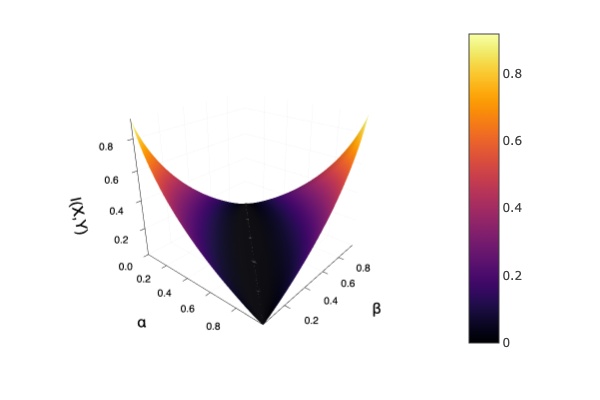
\includegraphics{img/I(X,Y).png}
\caption{plot of I(X,Y)}
\end{figure}

From the analysis and the plot, we can see that the mutual information
is maximal when \((\alpha, \beta) \in \{(0,0),(1,1)\}\). The capacity is
\(1\) bit.

\hypertarget{f-what-condition-do-alpha-beta-satisfy-when-the-capacity-of-this-channel-is-minimal-what-is-the-channel-capacity-in-that-case}{%
\subsubsection{\texorpdfstring{(f) What condition do \((\alpha, \beta)\)
satisfy when the capacity of this channel is minimal? What is the
channel capacity in that
case?}{(f) What condition do (\textbackslash alpha, \textbackslash beta) satisfy when the capacity of this channel is minimal? What is the channel capacity in that case?}}\label{f-what-condition-do-alpha-beta-satisfy-when-the-capacity-of-this-channel-is-minimal-what-is-the-channel-capacity-in-that-case}}

From the analysis and the plot, we can see that when \(\alpha+\beta=1\),
the mutual information is minimal. The capacity is \(0\) bit.

\hypertarget{principle-of-maximum-entropy}{%
\subsection{(4) Principle of Maximum
Entropy}\label{principle-of-maximum-entropy}}

\hypertarget{a-start-with-a-given-distribution-for-an-unfair-die-with-distribution-112-112-16-16-14-14.-calculate-the-best-guess-of-the-distribution-for-the-cases}{%
\subsubsection{(a) Start with a given distribution for an ``unfair'' die
with distribution \{1/12, 1/12 , 1/6, 1/6, 1/4, 1/4\}. Calculate the
best guess of the distribution for the
cases}\label{a-start-with-a-given-distribution-for-an-unfair-die-with-distribution-112-112-16-16-14-14.-calculate-the-best-guess-of-the-distribution-for-the-cases}}

\hypertarget{i-of-no-information}{%
\paragraph{(i) of no information}\label{i-of-no-information}}

It's esay to see that the best guess is the uniform distribution
\(p_i=1/6\).

\hypertarget{ii-the-case-of-knowing-only-the-average-sum_i16ip_ifrac256-.}{%
\paragraph{\texorpdfstring{(ii) the case of knowing only the average
\(\sum_{i=1}^6ip_i=\frac{25}6\)
.}{(ii) the case of knowing only the average \textbackslash sum\_\{i=1\}\^{}6ip\_i=\textbackslash frac\{25\}6 .}}\label{ii-the-case-of-knowing-only-the-average-sum_i16ip_ifrac256-.}}

Form the Lagrangian function:

\[
\begin{aligned}
L(p;\lambda_0,\lambda_1)=-\sum_{i=1}^6p_i\ln{p_i}
+\lambda_0\left(\sum_{i=1}^6p_i-1\right)+\lambda_1\left(\sum_{i=1}^6p_i-\frac{25}6\right)
\end{aligned}
\]

Take the derivative with respect to \(p_i\):

\[
\begin{aligned}
\frac{\partial L}{\partial p_i}
&=-1-\ln{p_i}+\lambda_0+i\lambda_1\\
\end{aligned}
\]

Set it to zero, then get:

\[
\begin{aligned}
p_i&=\exp(-1+\lambda_0+\lambda_1i)=\frac{e^{\lambda_1i}}{\sum e^{\lambda_1i}}\\
\end{aligned}
\]

Then solve the \(\lambda_0,\lambda_1\) by the constraint:

\[
\begin{aligned}
\sum_{i=1}^6p_i&=\exp(-1+\lambda_0)\sum ie^{\lambda_1i}=1\\
\sum_{i=1}^6ip_i&=\frac{\sum ie^{\lambda_1i}}{\sum e^{\lambda_1i}}=\frac{25}6\\
\end{aligned}
\]

Let \(a=e^{\lambda_1}\), then we get:

\[
\begin{aligned}
6\sum_{i=1}^6ia^i&=25\sum_{i=1}^6a^i\\
\sum_{i=1}^6 (6i-25)a^i&=0\\
11 a^6 + 5 a^5 - a^4 - 7 a^3 - 13 a^2 - 19 a &= 0\\
a&\approx 1.26661
\end{aligned}
\]

Then the \(\lambda_1=\ln1.26661\approx0.239\).

Then the distribution is:

\[
\begin{aligned}
p_i&=\frac{e^{\lambda_1i}}{\sum e^{\lambda_1i}}\\
&=\frac{e^{0.239i}}{\sum e^{0.239i}}\\
\end{aligned}
\]

\hypertarget{b-let-p_i-by-the-probabilities-of-a-particle-having-energy-level-epsilon_i-respectively-where-n-is-the-number-of-energy-levels-and-let-the-mean-value-of-energy-be-barepsilon.-by-maximizing-the-shannon-entropy}{%
\subsubsection{\texorpdfstring{(b) Let \(p_i\) by the probabilities of a
particle having energy level \(\epsilon_i\), respectively, where \(n\)
is the number of energy levels, and let the mean value of energy be
\(\bar\epsilon\). By maximizing the Shannon
entropy,}{(b) Let p\_i by the probabilities of a particle having energy level \textbackslash epsilon\_i, respectively, where n is the number of energy levels, and let the mean value of energy be \textbackslash bar\textbackslash epsilon. By maximizing the Shannon entropy,}}\label{b-let-p_i-by-the-probabilities-of-a-particle-having-energy-level-epsilon_i-respectively-where-n-is-the-number-of-energy-levels-and-let-the-mean-value-of-energy-be-barepsilon.-by-maximizing-the-shannon-entropy}}

\[
\begin{aligned}
H(p)=-\sum_{i=1}^np_i\ln{p_i}
\end{aligned}
\]

Subject to,

\[
\begin{cases}
\sum_{i=1}^np_i&=1\\
\sum_{i=1}^n\epsilon_ip_i&=\bar\epsilon\\
\end{cases}
\]

Form the Lagrangian function:

\[
\begin{aligned}
L(p;\lambda_0,\lambda_1)=-\sum_{i=1}^np_i\ln{p_i}
+\lambda_0\left(\sum_{i=1}^np_i-1\right)+\lambda_1\left(\sum_{i=1}^n\epsilon_ip_i-\bar\epsilon\right)
\end{aligned}
\]

Take the derivative with respect to \(p_i\):

\[
\begin{aligned}
\frac{\partial L}{\partial p_i}
&=-1-\ln{p_i}+\lambda_0+\epsilon_i\lambda_1\\
\end{aligned}
\]

Set it to zero, then get:

\[
\begin{aligned}
p_i&=\exp(-1+\lambda_0+\epsilon_i\lambda_1)=\frac{e^{\epsilon_i\lambda_1}}{\sum e^{\epsilon_i\lambda_1}}\\
\end{aligned}
\]

\begin{quote}
Since I am not a student in physics major, so I just follow the hint
that ``identify one of the Lagrange multiplier \(\lambda_1\) to be equal
to \(-1/kT\)''.
\end{quote}

Then get the distribution:

\[
\begin{aligned}
p_i&=\frac{e^{-\epsilon_i/kT}}{\sum e^{-\epsilon_i/kT}}\\
\end{aligned}
\]

Then, it's easy to get the mean value of energy:

\[
\begin{aligned}
\bar\epsilon&=\sum_{i=1}^n\epsilon_ip_i\\
&=\sum_{i=1}^n\epsilon_i\frac{e^{-\epsilon_i/kT}}{\sum e^{-\epsilon_i/kT}}\\
&=\frac{\sum_{i=1}^n\epsilon_ie^{-\epsilon_i/kT}}{\sum_{i=1}^n e^{-\epsilon_i/kT}}\\
\end{aligned}
\]
